\section{函数}

\begin{enumerate}
\def\labelenumi{\arabic{enumi}.}
\tightlist
\item
  设E和F是两个集合，它们可能相同也可能不同。E的变元x与F的变元y之间的关系称为关于y的函数关系，如果对于所有 \(x \in E\) ，存在唯一的 \(y \in F\) 与 x 具有给定关系。
\end{enumerate}

我们将这种将每个元素 \(x \in E\) 该元素 \(y \in F\) 与 x 具有给定关系的运算称为函数；y 称为函数在元素 x 处的值，而该函数称为由给定的函数关系所确定。两个等价的函数关系确定同一个函数。这样的函数被称为“取值于 F 中”且“定义在 E 上”。更简洁地说，它也被称为从 E 到 F 的映射。

\begin{enumerate}
\def\labelenumi{\arabic{enumi}.}
\setcounter{enumi}{1}
\tightlist
\item
  集合E到集合F的映射是某个新集合的元素，即从E到F的映射的集合。若f是该集合的任意元素，则f在E的元素x处的值通常记为 \(f(x)\) 。在某些情形下，记号 \(f_{x}\) (称为指标记号；此时集合E称为指标集)更为可取。关系“ \(y = f(x)\) ''是y中的函数关系，它决定了f。
\end{enumerate}

当一个形如 \(y = \langle x \rangle\) （其中 \(\langle x \rangle\) 表示一种符号的组合，其中 \(x\) 可能出现）的关系在 \(y\) 中是一个函数关系时，它所确定的函数通常用记号 \(x \to \langle x \rangle\) 表示，甚至简记为 \(\langle x \rangle\) ；这是非常常见的语言滥用。例如，如果 \(X\) 和 \(Y\) 是一个集合 \(E\) 的两个一般子集，关系 \(Y = \complement X\) 在 \(Y\) 中是函数性的；它所确定的 \(\mathfrak{P}(E)\) 到 \(\mathfrak{P}(E)\) 的映射记作 \(X \to \complement X\) ，或简称为 \(\complement X\) .

我们不说“设 f 为从 E 到 F 的映射”，而常常更简单地说“设 \(f: E \rightarrow F\) ''.

为了描述涉及多个映射的情形，我们还将使用诸如下图所示的图表：

\pandocbounded{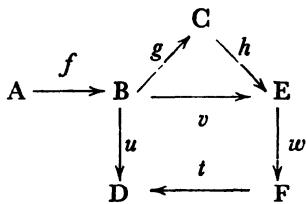
\includegraphics[keepaspectratio]{images/part003_3866b0bf02291d28d06ad2c75d3a73e7be589c55410c746bfd40818492cdc992.jpg}}

其中箭头旁标注的字母表示从箭头尾部集合到箭头头部集合的映射。

映射f=g（即E到F的映射相等）这一关系等价于“对所有 \(x \in E, f(x) = g(x)\) ''.

\begin{enumerate}
\def\labelenumi{\arabic{enumi}.}
\setcounter{enumi}{2}
\tightlist
\item
  定义在集合E上的函数，若对E中的每一个元素x都取相同的值a，则称为E上的常值函数；它由函数关系y = a确定。
\end{enumerate}

将E映入E的映射，它把E中的每个元素x与这个元素本身对应起来，称为恒等映射。它由函数关系y = x确定。

如果A是E的任意子集，则将A中每个元素x视为E中的同一元素而把A映入E的映射，称为A到E的典范映射。

让 \(f\) 是集合 \(\mathbf{E}\) 到自身的一个映射。一个元素 \(x\) （属于 \(\mathbf{E}\) ）被称为在 \(f\) 之下固定（或不变），如果 \(f(x) = x\) .

E 的元素 x 被称为在 E 到 E 的一组映射下固定（或不变），如果它在每个映射下都是固定的。

\begin{enumerate}
\def\labelenumi{\arabic{enumi}.}
\setcounter{enumi}{3}
\tightlist
\item
  让 \(f\) 是从 \(\mathbf{E}\) 到 \(\mathbf{F}\) 的映射，并令 \(\mathbf{X}\) 是 \(\mathbf{E}\) 的任意子集。则 \(\mathbf{X}\) 在 \(f\) 之下的像 \(\mathbf{Y}\) 是 \(\mathbf{F}\) 的一个子集 ，由所有元素 \(y\) （具有性质“存在 \(x \in \mathbf{E}\) 使得 \(x \in \mathbf{X}\) 并且 \(f(x) = y\)”）组成.
\end{enumerate}

这定义了X与Y之间的一种关系，该关系在Y上是函数性的，因此确定了从 \(\mathfrak{P}(\mathbf{E})\) 到 \(\mathfrak{P}(\mathbf{F})\) 的某个映射。该映射被称为 f 到子集集合的典范扩张；为简便起见，它也被记为f，我们写作 \(\mathbf{Y}=f(\mathbf{X})\) .

对于所有 \(f\) 并且 \(x\) 我们拥有

\[
f (\phi) = \phi \quad \text { 且 } \quad f (\{x \}) = \{f (x) \}.
\]

借用语言习惯，值 \(f(x)\) （ \(f\) 在 \(x\) 处的值）也被称为 \(x\) 在 \(f\) 之下的像.

如果 y 是 F 的一般元素，则性质“ \(y \in f(E)\) '' 可以表述为“y 具有以下形式 \(f(x)\) ''.

滥用语言，该像 \(f(\mathbf{E})\) （即 \(\mathbf{E}\) 在 \(f\) 之下的像）有时被称为 \(f\) 的像.

如果我们有 \(f(\mathbf{E}) = \mathbf{F}\) ，即如果对所有 \(y \in \mathbf{F}\) 存在 \(x \in \mathbf{E}\) 使得 \(y = f(x)\) ，那么 \(f\) 被称为从 \(\mathbf{E}\) 到 \(\mathbf{F}\) 上的映射，或满射映射，或满射。

让 \(x\) 是任意元素且 \(X\) 是 \(E\) 的任何子集。我们不说 \(f(x)\) 是 \(f\) 在 \(x\) 处的值、且 \(f(X)\) 是 \(X\) 在 \(f\) 之下的像，而是有时说 \(f\) 把 \(x\) 变换（或映射）为 \(f(x)\) ，把 \(X\) 变换为 \(f(X)\) ; \(f(x)\) 和 \(f(X)\) 则分别称为由 \(f\) 所给出的 \(x\) 和 \(X\) 的变换。

如果 f 是 E 到自身的一个映射，则称 E 的子集 X 在 f 下稳定，如果 \(f(\mathbf{X}) \subset \mathbf{X}\) 。如果 X 在 E 到 E 的映射集合中的每一个映射下都稳定，则称子集 X 在该映射集合下稳定。

\begin{enumerate}
\def\labelenumi{\arabic{enumi}.}
\setcounter{enumi}{4}
\tightlist
\item
  设 \(f\) 是从 \(\mathbf{E}\) 到 \(\mathbf{F}\) 的映射。于是我们有以下命题，其中 \(\mathbf{X}\) 和 \(\mathbf{Y}\) 表示 \(\mathbf{E}\) 的任意子集:
\end{enumerate}

\begin{enumerate}
\def\labelenumi{(\alph{enumi})}
\item
  关系 \(\mathbf{X} \subset \mathbf{Y}\) 蕴含 \(f(\mathbf{X}) \subset f(\mathbf{Y})\) .
\item
  该性质 \(\mathbf{X} \neq \emptyset\) 等价于 \(f(\mathbf{X}) \neq \emptyset\) .
\item
  对于所有 \(\tilde{\mathbf{X}}\) , \(\mathbf{Y}\) 我们拥有
\end{enumerate}

\begin{enumerate}
\def\labelenumi{(\arabic{enumi})}
\setcounter{enumi}{10}
\tightlist
\item
\end{enumerate}

\[
f (\mathbf {X} \cup \mathbf {Y}) = f (\mathbf {X}) \cup f (\mathbf {Y}),\tag{12}
\]

\[
f (\mathbf {X} \cap \mathbf {Y}) \subset f (\mathbf {X}) \cap f (\mathbf {Y}).
\]

\begin{enumerate}
\def\labelenumi{\arabic{enumi}.}
\setcounter{enumi}{5}
\tightlist
\item
  让 \(f\) 是从 \(\mathbf{E}\) 到 \(\mathbf{F}\) 的映射，并且让 \(\mathbf{Y}\) 是 \(\mathbf{F}\) 的任意子集。 \(\mathbf{Y}\) 在 \(f\) 之下的逆像 \(\mathbf{X}\) 是 \(\mathbf{E}\) 的一个子集 ，由所有元素 \(x\) （具有该性质 \(f(x) \in \mathbf{Y}\) ）组成.
\end{enumerate}

这定义了X与Y之间的一种关系，该关系在X上是函数性的，因此确定了从 \(\mathfrak{P}(\mathbf{F})\) 到 \(\mathfrak{P}(\mathbf{E})\) 的一个映射，称为 f 到子集集合上的逆扩张，并记作 \(\overline{f}^{1}\) ；因此我们写 \(\mathbf{X} = \overline{f}^{1}(\mathbf{Y})\) .

特别地，如果 \(y\) 是 \(F\) ，那么 \(f^{1}(\{y\})\) 将是所有 \(x \in E\) 使得 \(f(x) = y\) 。关系“ \(f(x) = y\) ”和“ \(x \in \overline{f}^{1}(\{y\})\) ”是等价的。借用语言习惯，我们常写 \(\overline{f}^{1}(y)\) 以代替 \(\overline{f}^{1}(\{y\})\) .

迹 \(X_{A}\) 子集X在E中对给定子集A的逆像是X在A到E的典范映射（第3节）下的原像。

\begin{enumerate}
\def\labelenumi{\arabic{enumi}.}
\setcounter{enumi}{6}
\tightlist
\item
  让 \(f\) 是从 \(\mathbf{E}\) 到 \(\mathbf{F}\) 的映射。于是我们有以下命题，其中 \(\mathbf{X}\) 和 \(\mathbf{Y}\) 表示 \(\mathbf{F}\) 的任意子集:
\end{enumerate}

\begin{enumerate}
\def\labelenumi{(\alph{enumi})}
\item
  关系 \(\mathbf{X} \subset \mathbf{Y}\) 蕴含 \(\overline{f}^1(\mathbf{X}) \subset \overline{f}^1(\mathbf{Y})\) .
\item
  对所有 X, Y，我们有
\end{enumerate}

\begin{enumerate}
\def\labelenumi{(\arabic{enumi})}
\setcounter{enumi}{12}
\tightlist
\item
\end{enumerate}

\[
\overline {{f}} ^ {1} (\mathrm{X} \cup \mathrm{Y}) = \overline {{f}} ^ {1} (\mathrm{X}) \cup \overline {{f}} ^ {1} (\mathrm{Y}),\tag{14}
\]

\[
\bar {f} ^ {1} (\mathrm{X} \cap \mathrm{Y}) = \bar {f} ^ {1} (\mathrm{X}) \cap \bar {f} ^ {1} (\mathrm{Y}),\tag{15}
\]

\[
\overline {{f}} ^ {1} (\mathbb {C X}) = \mathbb {C} \overline {{f}} ^ {1} (\mathbf {X}).
\]

注意公式(12)与(14)之间的区别；若将f替换为从F到E的任意映射，则(14)并非对所有X和Y都成立。同样，对于任意映射的扩张，不存在与(15)类似的结论。

此外，我们有 \(\overline{f}^{1}(\phi) = \phi\) ；但我们也可以有 \(\overline{f}^{1}(\mathbf{X}) = \phi\) ，其中 \(\mathbf{X}\) 是 \(\mathbf{F}\) 的一个非空子集. 为了使得 \(\mathbf{X} \neq \phi\) 蕴含 \(\overline{f}^{1}(\mathbf{X}) \neq \phi\) ，其充要条件是 \(f\) 是从 \(\mathbf{E}\) 到 \(\mathbf{F}\) 上的映射.

\begin{enumerate}
\def\labelenumi{\arabic{enumi}.}
\setcounter{enumi}{7}
\tightlist
\item
  如果映射 \(f\) （从 \(\mathbf{E}\) 到 \(\mathbf{F}\) 内的）满足对于所有 \(y \in \mathbf{F}\) 至多存在一个 \(x \in \mathbf{E}\) 使得 \(y = f(x)\) （换句话说，集合 \(\overline{f}^1(y)\) 要么为空，要么只包含一个元素），则 \(f\) 被称为从 \(\mathbf{E}\) 到 \(\mathbf{F}\) 内的一一映射，或单射映射，或单射。此时，对于所有子集 \(\mathbf{X}, \mathbf{Y}\) （ \(\mathbf{E}\) 的）,
\end{enumerate}

\[
f (\mathbf {X} \cap \mathbf {Y}) = f (\mathbf {X}) \cap f (\mathbf {Y}).\tag{16}
\]

\begin{enumerate}
\def\labelenumi{\arabic{enumi}.}
\setcounter{enumi}{8}
\tightlist
\item
  如果映射 \(f\) （从 \(\mathbf{E}\) 到 \(\mathbf{F}\) 内的）满足对于所有 \(y \in \mathbf{F}\) 恰好存在一个 \(x \in \mathbf{E}\) 使得 \(y = f(x)\) （换言之， \(\overline{f}(y)\) 由单一元素组成），则 \(f\) 被称为从 \(\mathbf{E}\) 到 \(\mathbf{F}\) 上的一一映射，或双射映射，或双射。这样的映射可以刻画为既是E到F上的映射，又是E到F内的一一映射。
\end{enumerate}

如果 \(f\) 是 \(\mathbf{E}\) 到 \(\mathbf{F}\) 上的一一映射，关系 \(y = f(x)\) 不仅在 \(y\) 中是泛函的，而且在 \(x\) 中也是泛函的。作为 \(x\) 中的泛函关系，它确定了 \(\mathbf{F}\) 到 \(\mathbf{E}\) 上的一个一一映射，称为映射 \(f\) 的逆映射.

注意，f 的逆的延拓与 f 的延拓的逆是相同的。

令 \(g\) 为 \(f\) 的逆。那么关系“ \(y = f(x)\) ”和“ \(x = g(y)\) '' 是等价的。\(g\) 的逆是 \(f\) 。如果 \(f\) 是 \(E\) 到 \(F\) 上的一一映射，我们不仅有关系式 (16)，而且对所有子集 \(X\) （ \(E\) 的）有

\[
f (\mathbf {C X}) = \mathbf {C} f (\mathbf {X}).
\]

此外， \(f\) 的扩张是 \(\mathfrak{P}(\mathbf{E})\) 到 \(\mathfrak{P}(\mathbf{F})\) 上的一一映射.

E到F的一一映射，连同其逆映射，称为实现E与F之间的一一对应；或者说，E与F通过这些映射被置于一一对应之中。

集合E到自身的一一映射称为E的一个置换。恒等映射是一个置换。若一个置换与其逆置换相同，则称其为对合的；例如，映射 \(X \rightarrow C X\) （ \(\mathfrak{P}(E)\) 到自身上的映射）是对合的。

\begin{enumerate}
\def\labelenumi{\arabic{enumi}.}
\setcounter{enumi}{9}
\tightlist
\item
  在以下命题中，X表示E的任意子集，Y表示F的任意子集：
\end{enumerate}

\begin{enumerate}
\def\labelenumi{(\alph{enumi})}
\tightlist
\item
  如果 \(f\) 是从 \(\mathbf{E}\) 到 \(\mathbf{F}\) 的映射，我们有
\end{enumerate}

\begin{enumerate}
\def\labelenumi{(\arabic{enumi})}
\setcounter{enumi}{16}
\tightlist
\item
\end{enumerate}

\[
\overline {{{f}}} ^ {1} (\mathrm{Y}) = \overline {{{f}}} ^ {1} (\mathrm{Y} \cap f (\mathrm{E})),\tag{18}
\]

\[
\mathbf {X} \subset \overline {{f}} ^ {1} (f (\mathbf {X})),\tag{19}
\]

\[
f (\overline {{f}} ^ {1} (\mathbf {Y})) \subset \mathbf {Y}.
\]

\begin{enumerate}
\def\labelenumi{(\alph{enumi})}
\setcounter{enumi}{1}
\item
  性质“对于所有Y， \(f(\bar{f}^{1}(Y)) = Y\) “f是E到F上的映射”与“f是E到F的满射”是等价的。
\item
  所有X都具有的性质， \(\overline{f}^{1}(f(X)) = X\) “f是E到F的一一映射”与“f是E到F的单射”是等价的。
\item
  对所有X和Y，
\end{enumerate}

\[
\bar {f} ^ {1} (f (\mathbf {X})) = \mathbf {X} \quad \text { 且 } \quad f (\bar {f} ^ {1} (\mathbf {Y})) = \mathbf {Y}"
\]

且“f是E到F上的一一映射”是等价的。

\begin{enumerate}
\def\labelenumi{\arabic{enumi}.}
\setcounter{enumi}{10}
\tightlist
\item
  设E、F、G为三个集合，它们可能相同也可能不同。设f为从E到F的映射，g为从F到G的映射。从E到G的映射，其在E中任一元素x处的值为 \(g(f(x))\) 称为g与f的复合，记作 \(g \circ f\) ，或在无歧义时简记为gf。
\end{enumerate}

这个等式 \(h = g \circ f\) 被称为 h 的一个分解。

注意，如果 G 与 E 不同，我们可能不能谈论 f 和 g 的复合（按此顺序），并且记号 \(f \circ g\) 没有意义。如果 G 与 E 相同，则 \(f \circ g\) 并且 \(g \circ f\) 不属于同一个集合，除非F也与E相同；即使如此，通常也是 \(f \circ g \neq g \circ f\) 。因此f和g的复合顺序是至关重要的。

令 \(\varphi\) 为 \(g\) 与 \(f\) 的复合，令 \(\mathbf{X}\) 是 \(\mathbf{E}\) 的任意子集，并且令 \(\mathbf{Z}\) 是 \(\mathbf{G}\) 的任意子集。于是我们有

\begin{enumerate}
\def\labelenumi{(\arabic{enumi})}
\setcounter{enumi}{19}
\tightlist
\item
\end{enumerate}

\[
\varphi (\mathbf {X}) = g (f (\mathbf {X})),\tag{21}
\]

\[
\overline {{{\varphi}}} ^ {1} (Z) = \overline {{{f}}} ^ {1} (\overline {{{g}}} ^ {1} (Z)).
\]

如果 \(f\) 是 \(\mathbf{E}\) 到 \(\mathbf{F}\) 上的一一映射，并且如果 \(g\) 是 \(\mathbf{F}\) 到 \(\mathbf{G}\) 上的一一映射，那么 \(g \circ f\) 是 \(\mathbf{E}\) 到 \(\mathbf{G}\) 上的一一映射.

让 \(h\) 是从 \(G\) 到一个集合 \(H\) 的映射。于是我们有

\[
h \circ (g \circ f) = (h \circ g) \circ f;
\]

的复合，这个从E到H的映射写作 \(h \circ g \circ f\) ，并称为三个映射 h、g、f 按此顺序的复合。多于三个映射的复合类似地定义。

如果 \(f\) 是 \(\mathbf{E}\) 到自身的映射，其迭代 \(f\) 被定义为映射 \(f^n\) ( \(n\) 为整数 \(\geqslant 1\) )（即 \(\mathbf{E}\) 到自身的映射），通过对 \(n\) 的归纳、借助于关系 \(f^1 = f\) , \(f^n = f^{n-1} \circ f\) 来定义； \(f^n\) 被称为 \(f\) 的n次迭代。我们有 \(f^{m+n} = f^m \circ f^n\) .

\begin{enumerate}
\def\labelenumi{\arabic{enumi}.}
\setcounter{enumi}{11}
\tightlist
\item
  一般来说，复合映射 \(\overline{f}^{1} \circ f\) （由一个映射 \(f\) 的逆扩张与扩张复合而成）并不是 \(\mathfrak{P}(\mathbf{E})\) 到自身的恒等映射。同样地， \(f \circ \overline{f}^1\) 通常也不是 \(\mathfrak{P}(\mathbf{E})\) 到自身的恒等映射。这两个条件同时成立，仅当 \(f\) 是 \(\mathbf{E}\) 到 \(\mathbf{F}\) 上的双射.
\end{enumerate}

如果 \(f\) 是 \(\mathbf{E}\) 到 \(\mathbf{F}\) 上的双射，并且如果 \(g\) 表示 \(f\) 的逆，则复合 \(g \circ f\) 与 \(f \circ g\) 分别是 \(\mathbf{E}\) 到 \(\mathbf{E}\) 上以及 \(\mathbf{F}\) 到 \(\mathbf{F}\) 上的恒等映射.

反之，如果 \(f\) 是从 \(\mathbf{E}\) 到 \(\mathbf{F}\) 的映射，以及 \(g\) 是从 \(\mathbf{F}\) 到 \(\mathbf{E}\) 的映射，使得 \(g \circ f\) 是 \(\mathbf{E}\) 的一个排列并且 \(f \circ g\) 是 \(\mathbf{F}\) 的一个排列，那么 \(f\) 是 \(\mathbf{E}\) 到 \(\mathbf{F}\) 上的双射并且 \(g\) 是 \(\mathbf{F}\) 到 \(\mathbf{E}\) 上的双射.

此外，如果 \(g \circ f\) 是 \(\mathbf{E}\) 到自身上的恒等映射，那么 \(g\) 是 \(f\) 的逆.

\begin{enumerate}
\def\labelenumi{\arabic{enumi}.}
\setcounter{enumi}{12}
\item
  设 \(f\) 是从 \(\mathbf{E}\) 到 \(\mathbf{F}\) 的映射，并设 \(\mathbf{A}\) 是 \(\mathbf{E}\) 的任意子集. 映射 \(f_{\mathbf{A}}\) （由 \(\mathbf{A}\) 到 \(\mathbf{F}\) ，其在任意元素 \(x\) （ \(\mathbf{A}\) 的）处的值为 \(f(x)\) ）称为 \(f\) 在子集 \(\mathbf{A}\) 上的限制；它就是 \(f\) 与由 \(\mathbf{A}\) 到 \(\mathbf{E}\) 的典范映射的复合. 如果两个映射 \(f, g\) （由 \(\mathbf{E}\) 到 \(\mathbf{F}\) ）在 \(\mathbf{A}\) 上的限制相同，则称它们在 \(\mathbf{A}\) 上一致. 反之， \(f\) 称为 \(f_{\mathbf{A}}\) 到 \(\mathbf{E}\) 的扩张.
\item
  将一个集合 E 映到集合 F 上的映射也称为 F 借助 E 的一个参数表示；此时 E 称为该表示的参数集，而 E 的元素则称为参数。
\end{enumerate}

集合 F 的一个元素族，按定义是 F 的一个子集连同其上的一个参数表示；换言之，给定 F 的一个元素族，等价于给定某个集合 E 到 F 的一个映射。E 在该映射下的像称为该族的元素集。注意，F 的两个不同的元素族可能具有相同的 F 的子集作为它们的元素集。

对于集合 F 的每个子集 A，我们总可以联系一个元素族，其元素集为 A。只需考虑由 A 到 F 的典范映射所定义的族即可。

由映射 \(\iota\to x_{i}\) 定义的 F 的元素族，记为 \((x_{i})_{i\in I}\) ，或简称为 \((x_{i})\) 如果关于指标集没有歧义的话。

如果 \(J\) 是 \(I\) 的子集，族 \((x_{t})_{t\in J}\) 被称为对应于 \(J\) 的子族（族 \((x_{t})_{t\in I}\) 的）；它由在 \(J\) 上限制映射 \(t\to x_t\) 而定义.

